\documentclass{article}
\usepackage{tikz}
\usetikzlibrary{arrows.meta,positioning,calc,shapes.geometric}
\pagestyle{empty}
\begin{document}
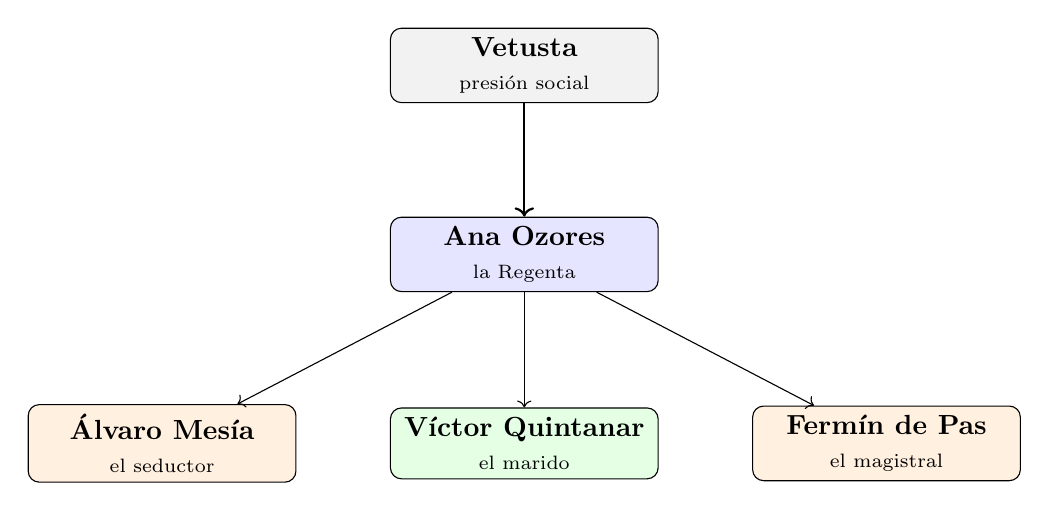
\begin{tikzpicture}
\tikzset{every node/.append style={align=center}}

\node[draw, rounded corners, fill=gray!10, minimum width=3.4cm, align=center] (v) at (0,2.4) {\textbf{Vetusta}\\ \scriptsize presión social};
\node[draw, rounded corners, fill=blue!10, minimum width=3.4cm, align=center] (a) at (0,0) {\textbf{Ana Ozores}\\ \scriptsize la Regenta};
\node[draw, rounded corners, fill=orange!12, minimum width=3.4cm, align=center] (m) at (-4.6,-2.4) {\textbf{Álvaro Mesía}\\ \scriptsize el seductor};
\node[draw, rounded corners, fill=orange!12, minimum width=3.4cm, align=center] (p) at (4.6,-2.4) {\textbf{Fermín de Pas}\\ \scriptsize el magistral};
\node[draw, rounded corners, fill=green!10, minimum width=3.4cm, align=center] (q) at (0,-2.4) {\textbf{Víctor Quintanar}\\ \scriptsize el marido};
\draw[->, thick] (v) -- (a); \draw[->] (a) -- (m); \draw[->] (a) -- (p); \draw[->] (a) -- (q);

\end{tikzpicture}
\end{document}
